\documentclass{article}
\usepackage[left=2.5cm,right=2.5cm, top = 2.5cm, bottom = 3cm]{geometry}


\begin{document}
\SweaveOpts{concordance=TRUE}

\title{A permutation-based comparison of ILI intensity thresholds from the moving epidemic and WHO methods}
\author{Johannes Bracher, Jonas Littek}

\maketitle


\abstract{The moving epidemic method (MEM) and the WHO method are widely used approaches to determine intensity levels for seasonal influenza and influenca-like illness (ILI). They are conceptually similar, but differ in two points. Firstly, the MEM involves a log-transformation of incidence data, while the WHO method operates on the original scale of the data. Secondly, the MEM method usually uses more than one observation from each past season, with the exact number depending on the number of available historical seasons. The WHO method, on the other side, uses only the single highest value from each past season. We perform a simulation study to assess the impact of these choices on the resulting intensity thresholds and empirical exceedance proportions. It is based on a permutation approach using historical ILI data from France, Spain, Switzerland and the United States.}

\section{Introduction}

\section{Definition of the moving epidemic and WHO methods}

\section{A brief review of recent applications}

Cite Benedetti who use it as a "gold standard". Mention Green GB who compare to percentile method. Vos mention fixed criterion model -- what is that?


\textbf{add table with Jonas' literature review here}

\section{Simulaton study}

\subsection{Permutation approach based on historical ILI data}

\subsection{Data}

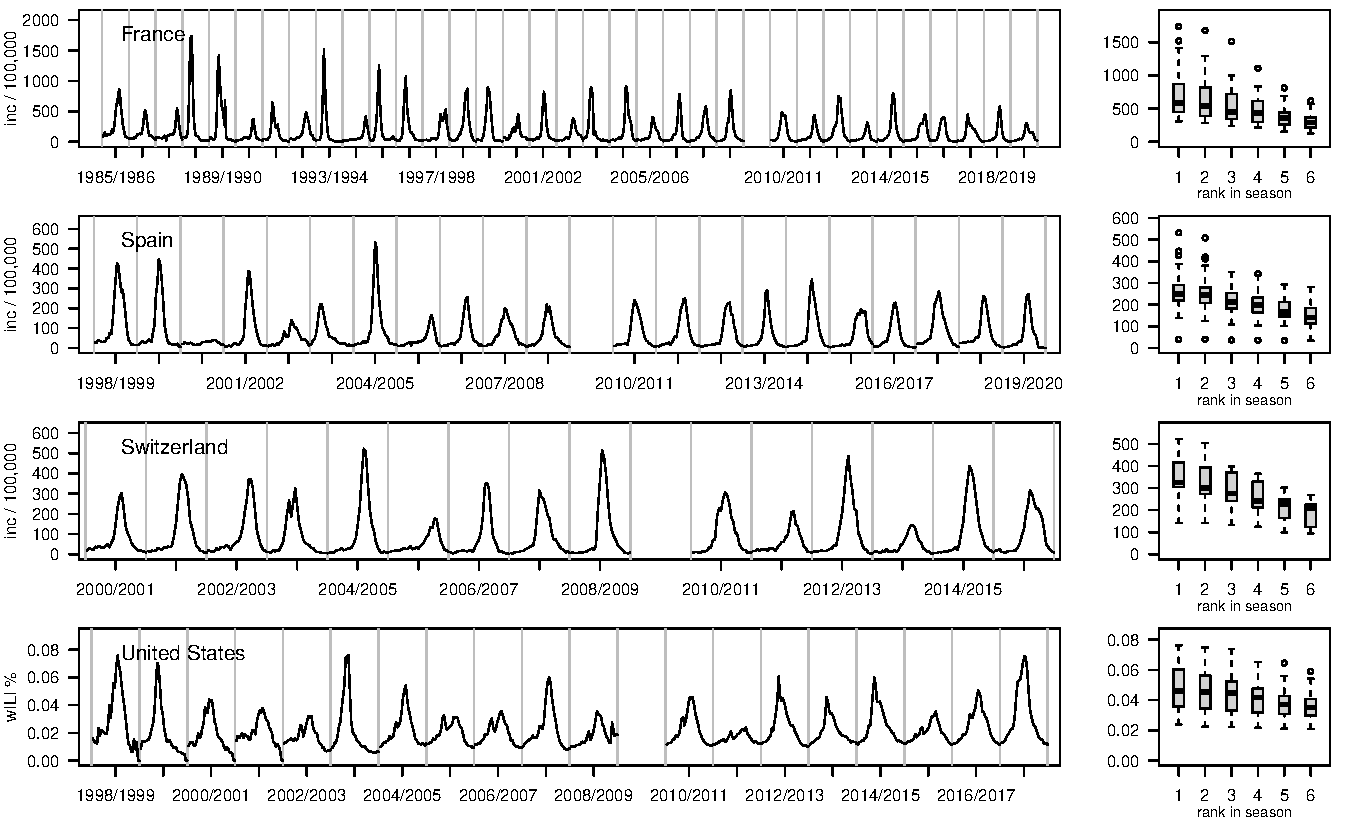
\includegraphics{figure/plot_data.pdf}

\subsection{Used software}

MEM version xxx, R software

\subsection{Results}

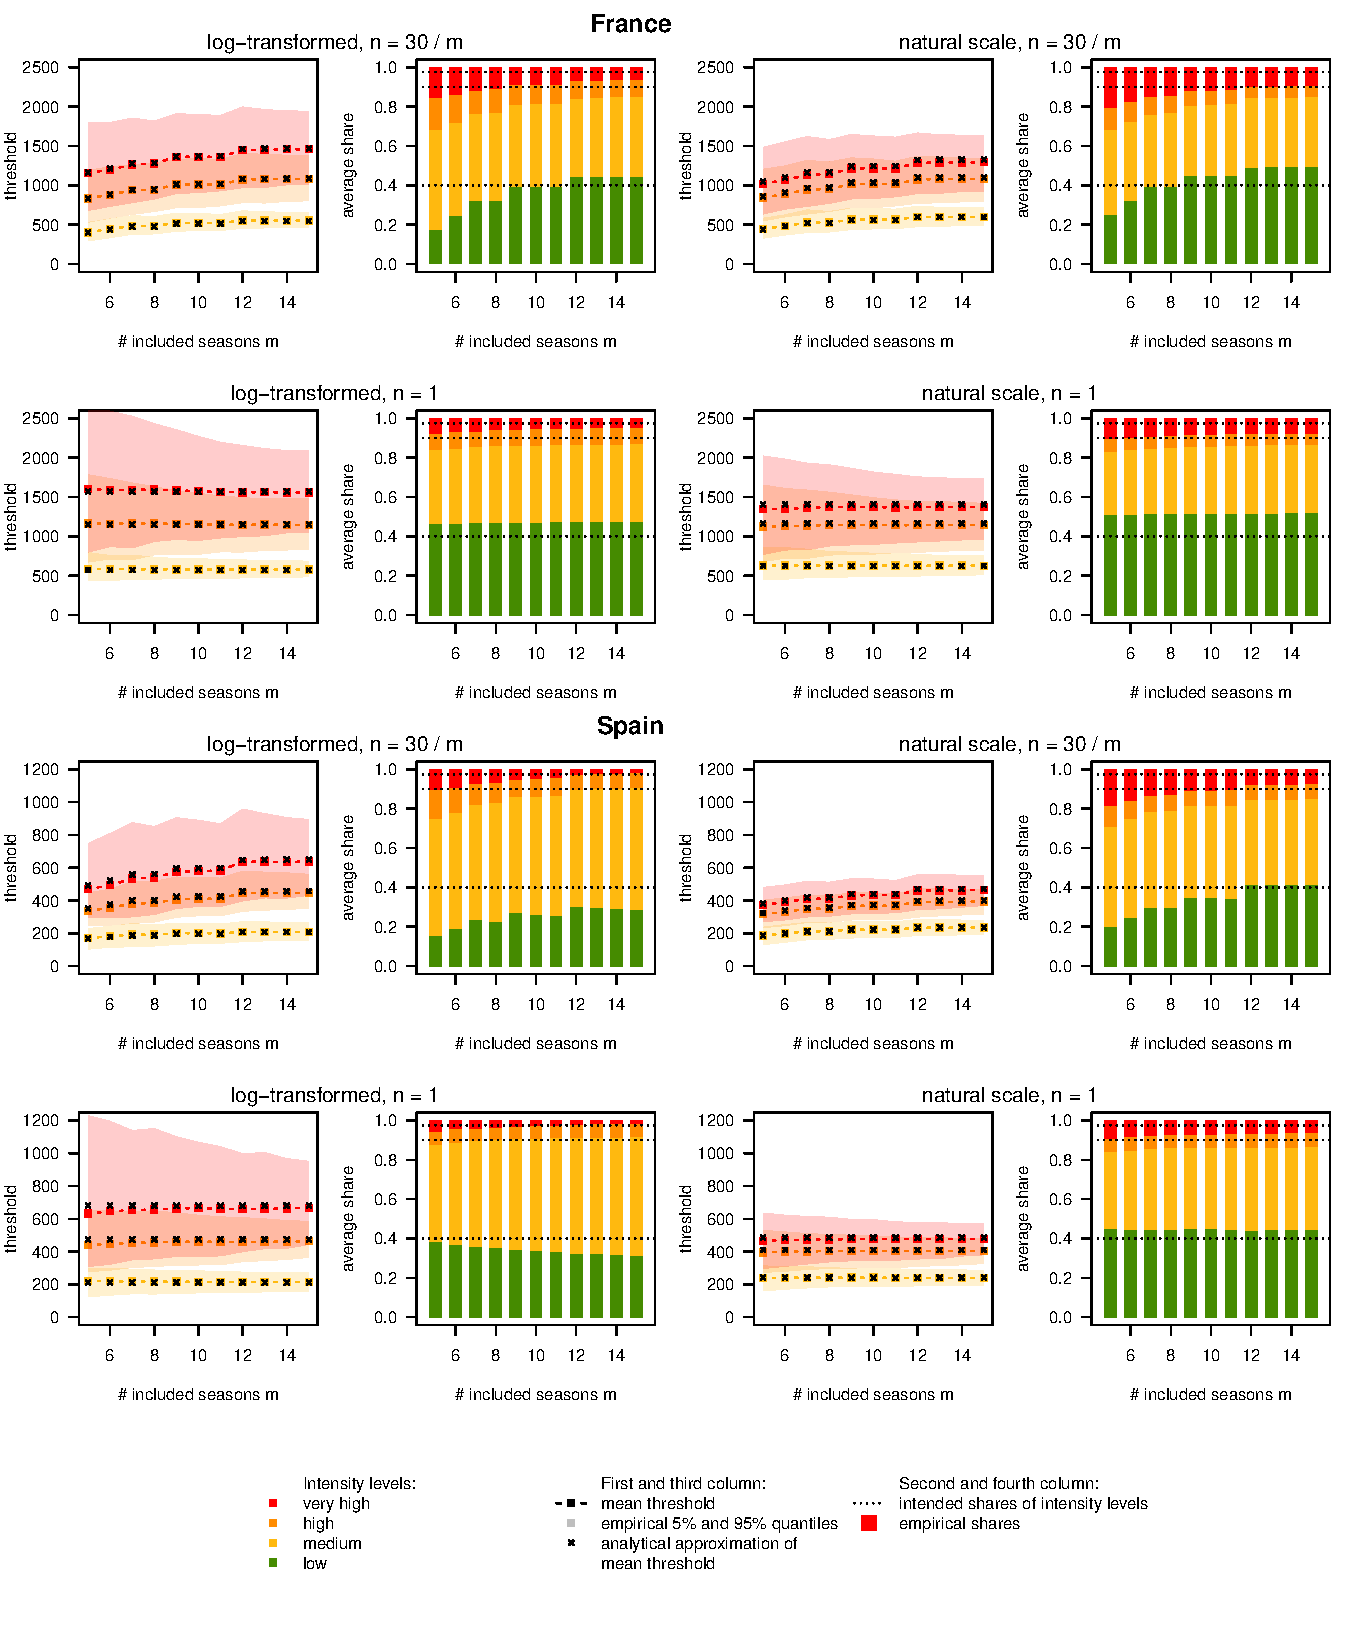
\includegraphics[page=1]{figure/plot_results.pdf}

\includegraphics[page=2]{figure/plot_results.pdf}


\section{Discussion}

\section*{Outline of idea}

\begin{itemize}
\item Description of importance: officially embraced by ECDC
\item Describe other approaches, in particular WHO
\item Statistically correct description of what is being done, contract to WHO approach (which only uses peak -- good -- but uses normal rather than log-normal -- not so good. There is a PLOS paper where there is already a kind of combination of the two (WHO with log transformation))
\item Overview of how it is being used in the literature:
\begin{itemize}
\item How much training data was available in each study?
\end{itemize}
\item Simulation study based on permutation of true seasons:
\begin{itemize}
\item Countries: France, Switzerland, some third (European) country? Spain?
\item Important: standardize with time-varying population
\end{itemize}
\end{itemize}

\title{A statistical perspective on the moving epidemic method }
\author{Johannes Bracher}
\maketitle




\bibliography{bibliography_mem}
\end{document}